\documentclass[tikz,border=3pt]{standalone}
\usepackage{amsmath}
\usetikzlibrary{arrows.meta,calc,positioning}
\definecolor{navy}{HTML}{173B57}
\definecolor{green}{HTML}{5B8F72}
\definecolor{orange}{HTML}{D9853B}
\definecolor{purple}{HTML}{6C5B8C}
\begin{document}
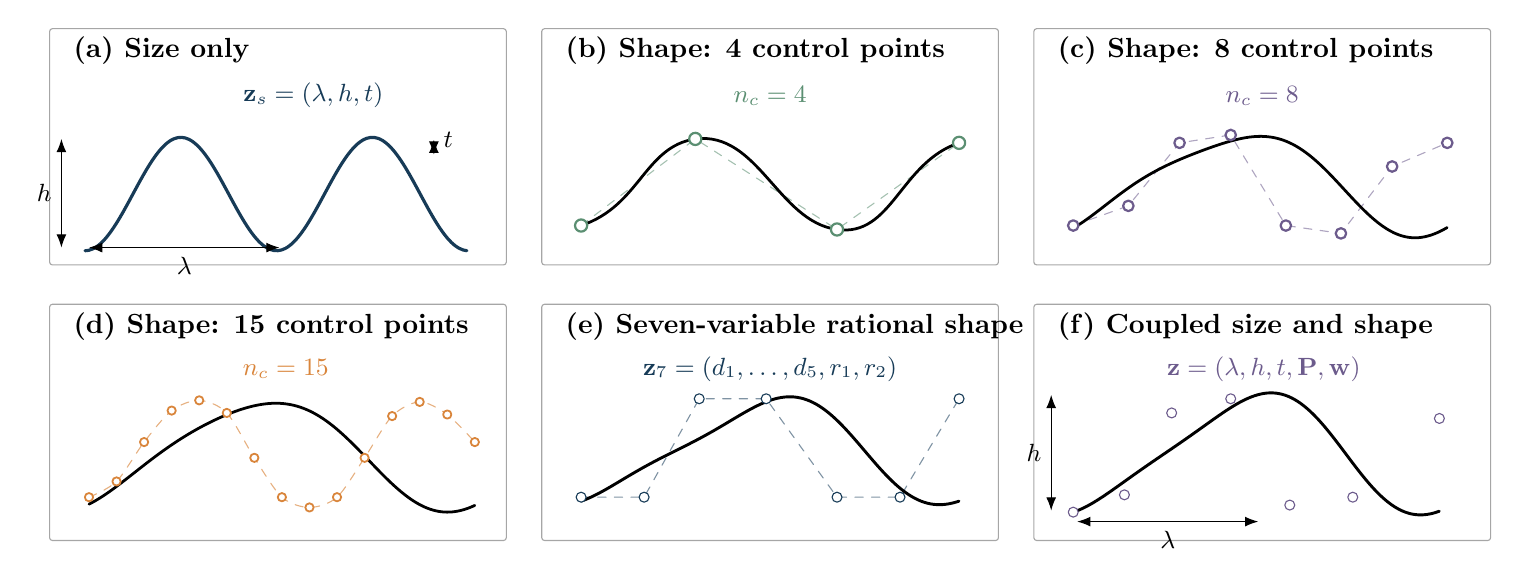
\begin{tikzpicture}[font=\small,>=Latex,line cap=round,line join=round]
  \tikzset{panel/.style={draw=black!35,rounded corners=1pt,minimum width=5.8cm,minimum height=3.0cm}}
  \foreach \cx/\cy/\title in {0/3.5/{(a) Size only},6.25/3.5/{(b) Shape: 4 control points},12.5/3.5/{(c) Shape: 8 control points},0/0/{(d) Shape: 15 control points},6.25/0/{(e) Seven-variable rational shape},12.5/0/{(f) Coupled size and shape}}{
    \node[panel] at ({\cx+2.9},{\cy+1.5}) {};
    \node[anchor=west,font=\bfseries] at ({\cx+0.18},{\cy+2.72}) {\title};
  }
  % Size only
  \draw[navy,line width=1.15pt,domain=0.45:5.3,samples=100,smooth]
    plot (\x,{4.4+0.72*sin(148*(\x-0.45)-90)});
  \draw[<->] (0.50,3.72)--(2.92,3.72) node[midway,below] {$\lambda$};
  \draw[<->] (0.15,3.72)--(0.15,5.10) node[midway,left] {$h$};
  \draw[<->] (4.88,4.90)--(4.88,5.09) node[right] {$t$};
  \node[navy] at (3.35,5.65) {$\mathbf z_s=(\lambda,h,t)$};
  % 4 CP
  \draw[green!55,dashed] (6.75,4.0)--(8.2,5.1)--(10.0,3.95)--(11.55,5.05);
  \draw[black,line width=1.0pt] (6.75,4.0)..controls (7.5,4.25) and (7.55,5.0)..(8.2,5.1)..controls (9.0,5.2) and (9.25,4.05)..(10.0,3.95)..controls (10.7,3.85) and (10.8,4.8)..(11.55,5.05);
  \foreach \x/\y in {6.75/4,8.2/5.1,10/3.95,11.55/5.05}{\filldraw[fill=white,draw=green,line width=0.8pt] (\x,\y) circle (2.2pt);}
  \node[green] at (9.15,5.65) {$n_c=4$};
  % 8 CP
  \draw[purple!55,dashed] (13.0,4.0)--(13.7,4.25)--(14.35,5.05)--(15.0,5.15)--(15.7,4.0)--(16.4,3.9)--(17.05,4.75)--(17.75,5.05);
  \draw[black,line width=1.0pt,domain=13:17.75,samples=120,smooth] plot (\x,{4.55+0.62*sin(76*(\x-13)-70)+0.11*sin(152*(\x-13))});
  \foreach \x/\y in {13/4,13.7/4.25,14.35/5.05,15/5.15,15.7/4,16.4/3.9,17.05/4.75,17.75/5.05}{\filldraw[fill=white,draw=purple,line width=0.8pt] (\x,\y) circle (1.9pt);}
  \node[purple] at (15.4,5.65) {$n_c=8$};
  % 15 CP
  \draw[orange!65,dashed] plot[smooth] coordinates {(0.5,0.55)(0.85,0.75)(1.2,1.25)(1.55,1.65)(1.9,1.78)(2.25,1.62)(2.6,1.05)(2.95,0.55)(3.3,0.42)(3.65,0.55)(4.0,1.05)(4.35,1.58)(4.7,1.76)(5.05,1.60)(5.4,1.25)};
  \draw[black,line width=1.0pt,domain=0.5:5.4,samples=140,smooth] plot (\x,{1.1+0.68*sin(73*(\x-0.5)-70)+0.08*sin(146*(\x-0.5))});
  \foreach \x/\y in {0.5/0.55,0.85/0.75,1.2/1.25,1.55/1.65,1.9/1.78,2.25/1.62,2.6/1.05,2.95/0.55,3.3/0.42,3.65/0.55,4/1.05,4.35/1.58,4.7/1.76,5.05/1.6,5.4/1.25}{\filldraw[fill=white,draw=orange,line width=0.65pt] (\x,\y) circle (1.5pt);}
  \node[orange] at (3.0,2.18) {$n_c=15$};
  % Seven-variable shape
  \draw[navy!55,dashed] (6.75,0.55)--(7.55,0.55)--(8.25,1.8)--(9.1,1.8)--(10.0,0.55)--(10.8,0.55)--(11.55,1.8);
  \draw[black,line width=1.05pt,domain=6.75:11.55,samples=120,smooth] plot (\x,{1.14+0.64*sin(75*(\x-6.75)-90)+0.13*sin(150*(\x-6.75))});
  \foreach \x/\y in {6.75/0.55,7.55/0.55,8.25/1.8,9.1/1.8,10/0.55,10.8/0.55,11.55/1.8}{\filldraw[fill=white,draw=navy] (\x,\y) circle (1.8pt);}
  \node[navy,align=center] at (9.15,2.18) {$\mathbf z_7=(d_1,\ldots,d_5,r_1,r_2)$};
  % Coupled
  \draw[black,line width=1.05pt,domain=13:17.65,samples=120,smooth] plot (\x,{1.10+0.74*sin(78*(\x-13)-90)+0.12*sin(156*(\x-13))});
  \draw[<->] (13.05,0.24)--(15.35,0.24) node[midway,below] {$\lambda$};
  \draw[<->] (12.72,0.38)--(12.72,1.85) node[midway,left] {$h$};
  \foreach \x/\y in {13/0.36,13.65/0.58,14.25/1.62,15/1.8,15.75/0.45,16.55/0.55,17.65/1.55}{\filldraw[fill=white,draw=purple] (\x,\y) circle (1.8pt);}
  \node[purple,align=center] at (15.42,2.18) {$\mathbf z=(\lambda,h,t,\mathbf P,\mathbf w)$};
\end{tikzpicture}
\end{document}
